\documentclass[11pt]{article}

\usepackage[margin=1in]{geometry}
\usepackage{amsmath}
\usepackage{graphicx}
\usepackage{booktabs}
\usepackage[hidelinks]{hyperref}

\title{Analytic State-Averaged DMRG-CASSCF Gradients and Nonadiabatic Couplings in a PySCF/pyblock2 Workflow}

\author{Author list to be finalized}
\date{\today}

\newcommand{\Eh}{E_{\mathrm{h}}}
\newcommand{\bfR}{\mathbf{R}}

\begin{document}

\maketitle

\begin{abstract}
Analytic nuclear gradients and nonadiabatic coupling vectors are central
ingredients for locating conical intersections and for propagating
nonadiabatic dynamics with multireference electronic-structure methods.
Complete-active-space self-consistent-field (CASSCF) theory provides a
robust reference near electronic degeneracies, but full configuration
interaction in the active space limits the accessible number of active
orbitals.  Here we report a PySCF/pyblock2 implementation of analytic
state-averaged density matrix renormalization group CASSCF
(SA-DMRG-CASSCF) gradients and nonadiabatic couplings, together with a
SHARC-compatible interface for requesting energies, dipoles, gradients, and
derivative couplings from the same workflow.  The implementation is validated
against PySCF full-CI active-space references on public benchmark systems.
We further quantify the finite-bond-dimension response error by replacing
FCI active-space vectors with block2 matrix product states at fixed
FCI-optimized orbitals.  The resulting convergence curves separate intrinsic
DMRG compression error from artifacts associated with reoptimizing orbitals in
a truncated CI manifold.  An ethylene interface regression test demonstrates
that the implemented DMRG-CASSCF backend writes all requested SHARC data
blocks.
\end{abstract}

\section{Introduction}

Nonadiabatic molecular processes require electronic-structure information
beyond adiabatic energies.  Surface-hopping algorithms and related
mixed quantum--classical methods use gradients and state couplings to
propagate nuclear motion through regions where the Born--Oppenheimer
separation breaks down.\cite{Tully1990,Richter2011SHARC,Mai2018SHARC}
For same-spin internal conversion, analytic derivative coupling vectors are
especially useful because they define, together with state gradients, the
first-order topology near conical intersections and provide direct inputs to
optimization and dynamics workflows.\cite{FdezGalvan2016}

CASSCF and state-averaged CASSCF (SA-CASSCF) wave functions are widely used
for this purpose because they provide a balanced multiconfigurational
description of near-degenerate states.  The conventional active-space solver,
however, is a full configuration interaction (FCI) expansion whose dimension
grows combinatorially with active electrons and orbitals.  The density matrix
renormalization group (DMRG) replaces the FCI vector by a matrix product state
(MPS), making compact approximations to much larger active spaces possible
when the entanglement structure is favorable.\cite{ChanHeadGordon2002,ChanSharma2011,SharmaChan2012}

Analytic response theory for DMRG-CASSCF has developed rapidly.  Freitag and
co-workers introduced an approximate SA-DMRG-SCF gradient and nonadiabatic
coupling formalism based on single-site MPS Lagrange multipliers in a
mixed-canonical representation.\cite{Freitag2019}  Iino, Shiozaki, and Yanai
later formulated analytic nuclear gradients for SA-DMRG-CASSCF using newly
derived coupled-perturbed equations.\cite{Iino2023}  These developments
establish the theoretical foundation for DMRG-based derivative calculations.
The remaining practical need addressed here is an open, reproducible
PySCF-based implementation with regression tests, public benchmark data, and
an interface usable by SHARC-style nonadiabatic dynamics workflows.

This work makes three contributions.  First, we implement two complementary
SA-DMRG-CASSCF response paths in a PySCF/pyblock2 environment: a native MPS
response class and a PySCF-compatible active-space solver wrapper.  Second,
we validate gradients and nonadiabatic couplings against FCI active-space
references and characterize the finite-bond-dimension response error on
public benchmark systems.  Third, we expose the validated backend through a
SHARC-compatible PySCF interface and demonstrate the complete output path on a
public ethylene test case.  The contribution is therefore an implementation,
validation, and reproducibility paper rather than a new derivation of the
underlying SA-DMRG response theory.

\begin{table}[t]
\centering
\small
\caption{Positioning of the present work relative to closely related methods
and software.}
\label{tab:positioning}
\begin{tabular}{p{0.24\textwidth}p{0.25\textwidth}p{0.42\textwidth}}
\toprule
Work or software & Scope & Relation to the present implementation \\
\midrule
SA-CASSCF derivative couplings\cite{FdezGalvan2016}
& Analytic CASSCF NAC theory and implementations
& Provides the FCI active-space response reference used for numerical
validation. \\
SA-DMRG-SCF response\cite{Freitag2019}
& Approximate analytic gradients and NACs with MPS response variables
& Provides the theoretical DMRG response framework followed here. \\
SA-DMRG-CASSCF gradients\cite{Iino2023}
& Coupled-perturbed equations for analytic SA-DMRG-CASSCF gradients
& Establishes an independent modern formulation; the present work emphasizes
open PySCF/pyblock2 integration and NAC/interface validation. \\
PySCF and block2\cite{Sun2018PySCF,Sun2020PySCF,Zhai2023Block2}
& Open electronic-structure and DMRG infrastructure
& Supplies the host CASSCF derivative code and the spin-adapted MPS backend. \\
SHARC\cite{Richter2011SHARC,Mai2018SHARC}
& Nonadiabatic dynamics driver and data interface
& Defines the Hamiltonian, dipole, gradient, and derivative-coupling output
contract tested in the ethylene regression case. \\
\bottomrule
\end{tabular}
\end{table}

\section{Theory and Algorithm}

\subsection{State-Averaged CASSCF Response}

For an SA-CASSCF wave function, the orbitals and active-space CI coefficients
are optimized for a weighted average of several electronic states.  Analytic
gradients and nonadiabatic couplings are obtained by differentiating a
Lagrangian that enforces stationarity with respect to orbital rotations and
active-space wave-function parameters.  The resulting coupled-perturbed
CASSCF equations determine the orbital-response multipliers that enter the
effective one- and two-particle density matrices used in the derivative
contractions.\cite{FdezGalvan2016,Freitag2019}

\subsection{DMRG Active-Space Representation}

In DMRG-CASSCF, each active-space state is represented by an MPS rather than
by an explicit FCI vector.  A finite bond dimension $M$ controls the rank of
the MPS approximation and therefore the accuracy of energies, density
matrices, gradients, and derivative couplings.  Following the SA-DMRG-SCF
response strategy of Freitag et al., the present implementation evaluates the
response quantities needed by PySCF's SA-CASSCF derivative machinery while
using pyblock2/block2 for the MPS representation and DMRG optimization.
\cite{Freitag2019,Zhai2023Block2}

\subsection{Bond-Dimension Response Error}

To isolate the effect of the MPS compression, we define a fixed-orbital
bond-dimension response error.  For each benchmark system we first converge a
standard SA-CASSCF calculation with an FCI active-space solver.  We then hold
the converged molecular orbitals fixed, run spin-adapted block2 DMRG in the
same active-space Hamiltonian at a selected bond dimension $M$, convert the
resulting MPS roots into the PySCF active-space representation, and recompute
analytic gradients and nonadiabatic couplings.  The error is measured against
the FCI active-space derivative at the same orbitals,
\begin{align}
\Delta_g(M) &= \left\|\nabla_{\bfR} E_0(M) -
              \nabla_{\bfR} E_0^{\mathrm{FCI}}\right\|_2,\\
\Delta_d(M) &= \min_{\sigma=\pm 1}
              \left\|\mathbf{d}_{01}(M) -
              \sigma \mathbf{d}_{01}^{\mathrm{FCI}}\right\|_2 ,
\end{align}
where the sign minimization removes the arbitrary global phase of the
electronic states.  This protocol avoids mixing the MPS compression error
with nonstationarity from orbital reoptimization on a deliberately truncated
CI manifold.

\section{Implementation}

The implementation is built on PySCF\cite{Sun2018PySCF,Sun2020PySCF} and
pyblock2/block2.\cite{Zhai2023Block2}  Two code paths are provided.  The
native \texttt{CPDMRGCASSCFResponseMPS} path keeps the response operations in
MPS form.  The \texttt{MPSAsFCISolver} path exposes a PySCF-compatible
active-space solver interface, allowing the same DMRG roots to be used by
PySCF's CASSCF gradient and nonadiabatic-coupling infrastructure.  The latter
path is the main regression-test target because it permits direct comparison
with standard FCI active-space calculations.

The workflow used in the public benchmarks is:
\begin{enumerate}
\item converge an SA(2)-CASSCF reference with PySCF and an FCI active-space
solver;
\item freeze the converged orbitals and construct the active-space
Hamiltonian in the same orbital basis;
\item optimize spin-adapted block2 MPS roots at the selected bond dimension;
\item align the MPS roots with the FCI reference by maximum overlap and
global phase;
\item evaluate energies, one- and two-particle density matrices, gradients,
and derivative couplings through the PySCF response interface; and
\item compare the resulting derivatives to the FCI active-space values at
identical orbitals.
\end{enumerate}

The SHARC-facing interface adds a PySCF template method,
\texttt{dmrg-casscf}.  When requested, the interface constructs a PySCF
CASSCF object, installs the DMRG-backed active-space solver, evaluates the
requested Hamiltonian, dipole, gradient, and derivative-coupling quantities,
and writes them in SHARC \texttt{QM.out} format.  The ethylene example in
this work is used as an end-to-end interface regression test.

\section{Computational Details}

All benchmark calculations used singlet state averaging over two roots with
equal weights.  The public systems are listed in Table~\ref{tab:systems}.
The bond-dimension response-error calculations used FCI-converged SA-CASSCF
orbitals as the fixed orbital basis.  Spin-adapted SU2 block2 DMRG was then
run at each selected bond dimension, and the resulting state vectors were
phase-aligned to the FCI reference before evaluating derivative errors.
Gradients are reported in m$\Eh$/Bohr and derivative couplings in atomic
units.

The FCI reference calculations used restricted Hartree--Fock orbitals
converged to $10^{-12}$, SA-CASSCF energy convergence of $10^{-10}$, and a
CASSCF gradient convergence threshold of $10^{-7}$.  The bond-dimension scan
used up to 30 DMRG sweeps and a sweep tolerance of $10^{-12}$ unless noted
otherwise.  The ethylene SHARC-interface regression test used an
SA(2)-DMRG-CASSCF(2,2)/STO-3G model with $M=60$, ten DMRG sweeps, a DMRG
sweep tolerance of $10^{-8}$, CASSCF energy convergence of $10^{-8}$, and
CASSCF gradient convergence of $10^{-5}$.  These settings are intentionally
small enough for a public regression test and are not used to make a
mechanistic chemistry claim.

\begin{table}[h]
\centering
\caption{Public validation and benchmark systems.}
\label{tab:systems}
\begin{tabular}{llll}
\toprule
System & Basis & Active space & Role \\
\midrule
H$_4$ chain & STO-3G & CAS(4,4) & Small-system response validation \\
H$_2$O & STO-3G & CAS(4,4) & Small-system response validation \\
N$_2$ & STO-3G & CAS(6,6) & Medium-active-space response validation \\
H$_2$O & 6-31G & CAS(6,6) & NAC convergence benchmark \\
C$_2$ & STO-3G & CAS(8,8) & Larger active-space benchmark \\
LiF & STO-3G & CAS(4,4) & Nonzero-NAC benchmark \\
Ethylene & STO-3G & CAS(2,2) & SHARC-interface regression test \\
\bottomrule
\end{tabular}
\end{table}

\section{Results and Discussion}

\subsection{Validation Against FCI Active-Space References}

The implementation is covered by unit and integration tests for DMRG/FCI
energies, one- and transition-density matrices, MPS-to-FCI conversion,
analytic gradients, analytic derivative couplings, and SHARC output
formatting.  The current regression suite contains 46 passing tests across
14 test files.  These tests verify both direct numerical agreement with FCI
active-space references in small active spaces and consistency between the
native MPS and PySCF-compatible solver paths.

\begin{table}[t]
\centering
\small
\caption{Validation layers included in the public test and benchmark suite.}
\label{tab:validation}
\begin{tabular}{p{0.25\textwidth}p{0.32\textwidth}p{0.34\textwidth}}
\toprule
Validation target & Public evidence & Quantity checked \\
\midrule
DMRG active-space solver
& Solver regression tests
& Energies, state density matrices, transition density matrices, and analytic
NAC pipeline consistency with FCI references. \\
MPS/FCI mapping
& Active-space map tests
& Round-trip mapping for CAS(2,2), CAS(4,4), and CAS(8,8) active spaces. \\
Response linear algebra
& Coupled-perturbed response tests
& Hermiticity, linearity, response-vector solves, and agreement between MPS
and FCI response operations in exactly recoverable cases. \\
Gradient and NAC derivatives
& Derivative regression tests
& Analytic gradients and derivative couplings against PySCF FCI active-space
references. \\
SHARC interface
& Ethylene interface regression
& Presence of \texttt{H}, \texttt{DM}, \texttt{GRAD}, and \texttt{NACDR}
blocks in \texttt{QM.out} with SHARC master error code 0. \\
\bottomrule
\end{tabular}
\end{table}

\subsection{Finite-Bond-Dimension Response Error}

Figure~\ref{fig:bvoe} shows the fixed-orbital bond-dimension response error.
The H$_4$, H$_2$O/STO-3G, N$_2$, and H$_2$O/6-31G curves show systematic
decay of the derivative error as $M$ is increased.  The CAS(8,8) C$_2$ system
is a more demanding benchmark; it improves substantially with $M$ but also
shows the expected sensitivity of excited-state tracking in a compact
benchmark.  LiF provides a nonzero derivative-coupling test case.  Its energy
and gradient errors converge rapidly, whereas the derivative coupling remains
more gauge-sensitive, so it is interpreted as a diagnostic benchmark rather
than the primary convergence example.

The key observation is that the catastrophic response spikes observed with an
earlier SVD-truncated CI-vector proxy disappear when real DMRG roots are
evaluated at FCI-stationary orbitals.  This supports the interpretation that
those spikes were not intrinsic failures of the DMRG response approximation,
but artifacts of using a nonstationary truncated-CI orbital manifold.

\begin{table}[t]
\centering
\small
\caption{Representative largest-$M$ fixed-orbital response errors from the
public benchmark scan.}
\label{tab:largestm}
\begin{tabular}{lllll}
\toprule
System & Active space & $M$ & $\Delta_g$ (m$\Eh$/Bohr) & $\Delta_d$ \\
\midrule
H$_4$/STO-3G & CAS(4,4) & 12 & $8.99\times10^{-11}$ & $2.22\times10^{-7}$ \\
H$_2$O/STO-3G & CAS(4,4) & 12 & $1.44\times10^{-3}$ & $2.29\times10^{-6}$ \\
N$_2$/STO-3G & CAS(6,6) & 30 & $4.58\times10^{-1}$ & $3.72\times10^{-3}$ \\
H$_2$O/6-31G & CAS(6,6) & 30 & $9.37\times10^{-5}$ & $1.48\times10^{-4}$ \\
C$_2$/STO-3G & CAS(8,8) & 70 & $1.80$ & $5.70\times10^{-2}$ \\
LiF/STO-3G & CAS(4,4) & 12 & $1.75\times10^{-6}$ & $2.91\times10^{-1}$ \\
\bottomrule
\end{tabular}
\end{table}

\begin{figure}[h]
\centering
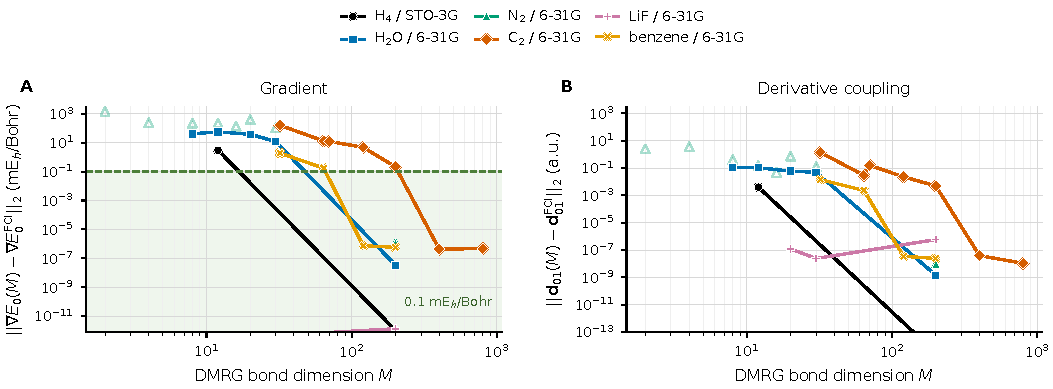
\includegraphics[width=\textwidth]{../benchmarks/bvoe_convergence_study/figures/bvoe_phase2.pdf}
\caption{Fixed-orbital bond-dimension response-error convergence for public
benchmark systems.  Gradient errors are reported in m$\Eh$/Bohr and
nonadiabatic coupling errors in atomic units.}
\label{fig:bvoe}
\end{figure}

\subsection{SHARC Interface Regression Test}

The public ethylene test requests the Hamiltonian, dipole matrices,
gradients for both singlet states, and the $S_0/S_1$ derivative coupling.
The calculation completes with SHARC master error code 0 and writes all
requested data blocks to \texttt{QM.out}.  This confirms that the DMRG-backed
PySCF object satisfies the data contract expected by the SHARC interface for
energies, dipoles, gradients, and derivative couplings.

\section{Conclusions}

We have implemented analytic SA-DMRG-CASSCF gradients and nonadiabatic
couplings in a PySCF/pyblock2 workflow and exposed the backend through a
SHARC-compatible PySCF interface.  The implementation is validated against
FCI active-space references, and public benchmark data quantify how gradient
and derivative-coupling errors decay with DMRG bond dimension at fixed
FCI-optimized orbitals.  The results provide a reproducible open-source
platform for testing DMRG-based multireference response quantities and for
connecting them to nonadiabatic dynamics interfaces.

\section*{Supporting Information}

Supporting Information: benchmark inputs, full convergence tables,
regression-test summary, and SHARC ethylene interface example files.

\section*{Data and Code Availability}

The public code bundle contains the response implementation, tests, benchmark
drivers, benchmark summaries, plotting scripts, and the ethylene SHARC
interface regression example.  A permanent repository URL or DOI should be
inserted in this section before journal submission.  Application systems and
trajectory data outside the public benchmark set are not included.

\section*{Acknowledgments}

Acknowledgments to be added.

\bibliographystyle{unsrt}
\bibliography{references}

\end{document}
